\chapter{Implementação do sistema}
%no capítulo de implementação é para mostrar como se fez. devem aparecer visualizações relacionas com o desenvolvimento, tais como classes ou diagramas da bd. Não é para usar o estilo documental de um relatório técnico, mas sim mais para enumerar as escolhas e dar algum enquadramento porque é que foi essa a escolha.

\section{Implementação e adaptação do backend}
% podem ser outras as subsecções; estas são ilustrativas. A idei é discutir as opções concretas tomadas para a implementação e os artifacts criados
\subsection{Servidor de Autorização e Autenticação}
O servidor de autenticação e autorização disponibiliza uma \gls{API} para criação de novos utilizadores e solicitação de tokens de acesso relativamente a várias aplicações. Este serviço utiliza a framework Spring, mais concretamente a Spring Security \cite{spring-framework}. \par 
No nosso caso vamos apenas ter uma aplicação cliente configurada para posteriormente gerir os tokens de acesso para esta aplicação. As credenciais das aplicações cliente vão estar guardadas num base de dados relacional e os utilizadores finais numa base de dados não relacional. Esta opção está relacionada com a proteção de dados referida anteriormente em \ref{cap6:protecaodados}. 
Relativamente à base de dados não relacional os utilizadores finais são guardados numa coleção do Mongo, a coleção é denominada por ''endUser''. Este coleção é então composta por vários documentos, em que cada documento corresponde a um utilizador final. Os documentos são formatados como na Figura \ref{f:endUserCode}

\begin{figure}[H]
\inputminted[fontsize=\scriptsize]{json}{code/endUser.json}
\caption[Formato do documento de um utilizador final]{Formato do documento de um utilizador final}
\label{f:endUserCode}
\end{figure}

Para a base de dados relacional a escolha podia por exemplo ser efetuada entre o MySQL \cite{mysql} e PostgreSQL \cite{postgresql}, neste caso foi utilizado o PostgreSQL, o modelo de dados relacional está representado na Figura \ref{f:auth-diagram}. \par 
Na tabela ''oauth\_client\_details'' estão guardadas todas as informações relativas à aplicação como por exemplo a sua identificação, a chave secreta, os tipos de autorização, etc. Relativamente à tabela ''oauth\_access\_token'' estão guardados os tokens de acesso por utilizador, relativamente a uma aplicação. Cada token de acesso tem relacionado a ele  um refresh token que está guardado numa tabela diferente, na tabela ''oauth\_refresh\_token''.

 \begin{figure}[H]
  \centering
  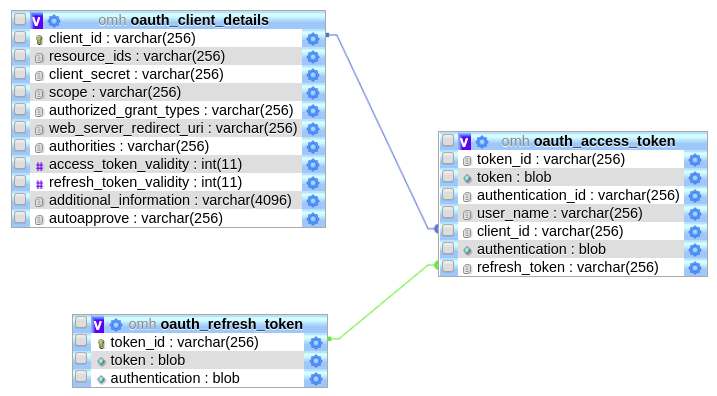
\includegraphics[width=0.8\textwidth]{imgs/auth-diagram.png}
  \caption[Diagrama do modelo de dados para guardar as credenciais dos clientes e os tokens de acesso]{Diagrama do modelo de dados para guardar as credenciais dos clientes e os tokens de acesso}
  
  \label{f:auth-diagram}
\end{figure}

\subsubsection{API REST}
\label{l:restapiAUTH}
Na tabela seguinte temos disponível os métodos disponíveis do servidor de autorização e autenticação.
\begin{table}[H]
\label{t:apirest-auth}
\centering
\begin{tabularx}{1\textwidth}{|p{0.3cm} p{14.4cm}|}
\multicolumn{2}{l}{\textbf{domain:port/users}}  \\ \hline 
 & Serviço POST, para criação de novos utilizadores \\
 & Recebe um JSON composto por dois campos um ''username'' e ''password'' \\ \hline
\multicolumn{2}{l}{\textbf{domain:port/oauth/token}} \\ \hline
 & Serviço POST, utilizado para efetuar o pedido de um novo token de acesso \\
 & Recebe por parâmetros o ''username'', ''password'' e o ''grant\_type'' \\ \hline
\end{tabularx}
\caption{Tabela com a API REST do servidor de autorização e autenticação}
\end{table}

\subsection{Servidor de recursos (dataPoint REST API) }
O servidor de recursos disponibiliza uma \gls{REST} \gls{API} para criação, consulta e eliminação de dataPoints. Estes dataPoints estão a ser guardados numa base de dados Mongo numa coleção com o nome dataPoint. A maior vantagem de utilizar uma base de dados não relacional é que os esquemas de dados podem ser extendidos à vontade que não é necessário efetuar nenhuma alteração ao esquema da BD. \par 
Como foi referido na fase exploratória do \gls{OMH} \ref{cap4:exp-omh} estes dataPoints são compostos por um cabeçalho e por um corpo. Este corpo é formatado pelo esquema de dados (dataschema) associado e definido no cabeçalho do dataPoint. Como foi referido também na fase exploratória foi desenvolvido um validador que verifica se o corpo do dataPoint está de acordo com o dataschema definido no cabeçalho do mesmo. \par
Estava então em falta alguns esquemas de dados para conseguirmos abranger todos os dados que precisávamos de inserir, assim como: \gls{ECG}, dados demográficos e acelerómetro. Estes dataschemas foram criados com base da informação retirada da definição da \gls{API} do \gls{FHIR} e vou mostrar de seguida como exemplo o esquema de dados criado para definir o formato de dados para as entradas para o \gls{ECG}. \newpage
\subsubsection{dataschema ECG}
\begin{figure}[H]
\inputminted[fontsize=\scriptsize]{json}{code/ecg.json}
\caption[Novo esquema de dados relativo ao ECG]{Novo esquema de dados relativo ao ECG}
\label{f:ecgjsonschema}
\end{figure}

\subsubsection{API REST}
\label{l:restapiRESOURCES}

\begin{table}[H]
\label{t:apirest-data}
\centering
\begin{tabularx}{1\textwidth}{|p{0.3cm} p{14.4cm}|}
\multicolumn{2}{l}{\textbf{domain:port/v\{apiVersion\}/dataPoints}}  \\ \hline 
 & Serviço POST, para criação de novos dataPoints \\
 & No header recebe o access\_token para o servidor de autorização para lhe dar acesso ao pedido efetuado \\
 & Recebe um documento JSON constituído por um cabeçalho e um corpo \\ \hline
\multicolumn{2}{l}{\textbf{domain:port/v\{apiVersion\}/dataPoints/id}} \\ \hline
 & Serviço DELETE, utilizado para efetuar a eliminação de um dataPoint \\
 & No header recebe o access\_token para o servidor de autorização para lhe dar acesso ao pedido efetuado \\
 & O id do dataPoint tem que ser referido no url \\ \hline
 \multicolumn{2}{l}{\textbf{domain:port/v\{apiVersion\}/dataPoints/id}} \\ \hline
 & Serviço GET, utilizado para efetuar a consulta de um dataPoint \\
 & No header recebe o access\_token para o servidor de autorização para lhe dar acesso ao pedido efetuado \\
 & O id do dataPoint tem que ser referido no url \\ \hline
 \multicolumn{2}{l}{\textbf{domain:port/v\{apiVersion\}/dataPoints/caregiver}} \\ \hline
 & Serviço GET, utilizado para efetuar a consulta dos vários dataPoints de um determinado tipo de um utilizador em específico \\
 & No header recebe o access\_token para o servidor de autorização para lhe dar acesso ao pedido efetuado \\
 & Recebe por parâmetros o ''schema\_namespace'', ''schema\_name'', ''schema\_version'', ''user\_id'' e o ''CAREGIVER\_KEY'' \\ \hline
 \multicolumn{2}{l}{\textbf{domain:port/v\{apiVersion\}/dataPoints}} \\ \hline
 & Serviço GET, utilizado para efetuar a consulta dos vários dataPoints de um determinado esquema de dados \\
 & No header recebe o access\_token para o servidor de autorização para lhe dar acesso ao pedido efetuado \\
 & Recebe por parâmetros o ''schema\_namespace'', ''schema\_name'' e o ''schema\_version'' \\ \hline
\end{tabularx}
\caption{Tabela com a API REST do servidor de recursos}
\end{table}


Todos os esquemas de dados disponíveis estão no diretório \cite{schemas-available} e estes são os tipos de dados que são utilizados para validar os dataPoints inseridos, ou seja, estes são todos aqueles que podem ser inseridos na coleção do Mongo.

\subsection{Comunicação com módulos externos}
No processo de inserção de novos dataPoints, depois de validados eles são reencaminhados para um endpoint \gls{REST}. É enviado um documento \gls{JSON} composto pelo esquema de dados utilizado para validar o documento, como por exemplo "heart-rate" e um corpo do dataPoint inserido. Este documento é então inserido no ''EventBus'' do Vert.x, neste momento os módulos que subscreberam o esquema de dados ''heart-rate'' pode verificar e analisar da maneira que quiser os dados inseridos. Temos na figura \ref{f:toExtSeqDiagram} um diagrama de sequência com este fluxo. \par
Isto pode ser importante para por exemplo ser desenvolvido um módulo que tenha a capacidade de verificar se um utilizador que está a fazer a colheita dos dados está a sofrer de Arritmia cardíaca.
O projeto é então composto por dois verticles em que num dois verticles cria um endpoint \gls{REST} e permite publicar os mesmo Eventbus assim que os recebe.

\begin{figure}[H]
  \centering
  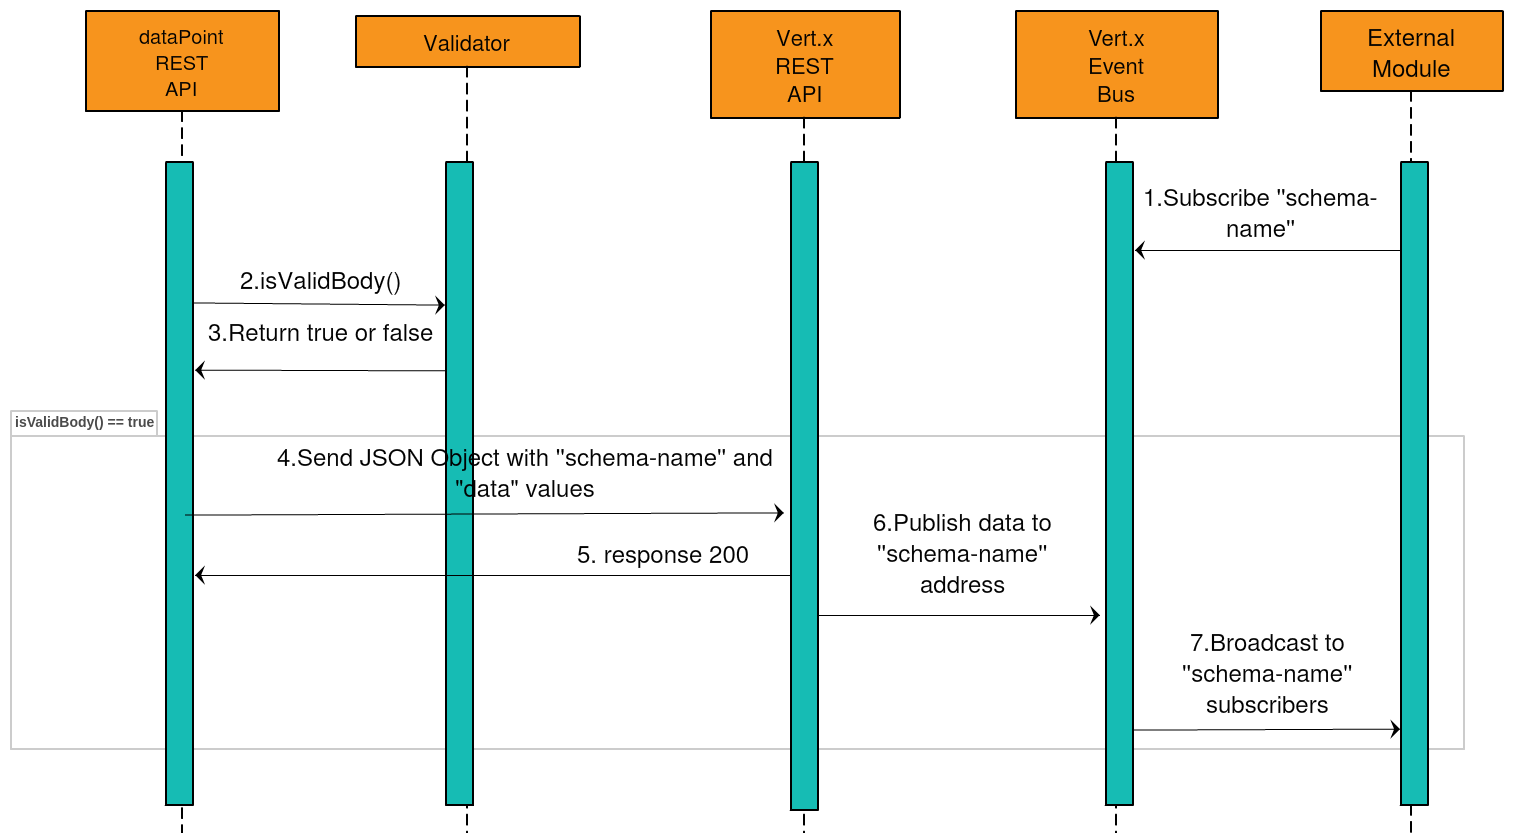
\includegraphics[width=1\textwidth]{imgs/toExtSeqDiagram.png}
  \caption[Diagrama de sequência com a comunicação com módulos externos]{Diagrama de sequência com a comunicação com módulos externos}
  
  \label{f:toExtSeqDiagram}
\end{figure}

\subsection{Como instalar este backend}
Relativamente ao servidor de autorização/autenticação e ao servidor de recursos o código está no github \cite{omh-code} e é um ''fork'' do projeto desenvolvido pela \gls{OMH}, está documentado como pode ser instalado e executado \cite{omh-runnatively}.
O código relativo à extensibilidade com módulos externos também está no github\cite{restpubsub} este projeto é composto apenas por dois verticles para os correr pode ser também por terminal e basta correr os comandos:
\begin{itemize}
    \item vertx run SimpleREST.java -cluster
    \item vertx run Receiver.java -cluster
\end{itemize}
O Receiver.java pode ser substituído ou adicionado por um outro módulo desenvolvido para receber outro tipo de esquemas de dados e os analisar.

\section{Implementação da aplicação móvel}
\subsection{Versões alvo e dependências}
Esta aplicação móvel foi desenvolvida com o intuito de conseguir abranger grande maioria dos utilizadores, suporta da versão 16 à versão 25, ou seja,  desde o Android 4.1 (Jelly Bean) até ao Android 7.1. De acordo com as informações disponíveis na plataforma de desenvolvimento do Android atinge mais de 98\% dos utilizadores \cite{android-versions}.

O projeto tem um ficheiro por defeito designado por "build.gradle", que é o local onde é efetuada a configuração relativa às versões alvo e às dependências existentes, um excerto deste ficheiro de configuração pode ser visualizado na tabela \ref{t:defaultconfigversions} e na tabela \ref{t:defaultconfigdependency} .


\begin{table}[H]
\centering
\begin{tabular}{|llll|}
\hline
 & \multicolumn{2}{l}{defaultConfig \{}                                     &  \\
 &    & applicationId {\color[HTML]{009901} ''pt.ua.ieeta.healthintegration''}                       &  \\
 &    & minSdkVersion {\color[HTML]{0767D2}16}                                                    &  \\
 &    & targetSdkVersion {\color[HTML]{0767D2}25}                                                 &  \\
 &    & versionCode {\color[HTML]{0767D2}1}                                                       &  \\
 &    & versionName {\color[HTML]{009901}''1.0''}                                                   &  \\
 & \} &                                                                     & \\
\hline
\end{tabular}
\caption[Excerto da configuração padrão da aplicação móvel relativo às versões]{Excerto da configuração padrão da aplicação móvel relativo às versões}
\label{t:defaultconfigversions}
\end{table}

\begin{table}[H]
\centering
\begin{tabular}{|llll|}
\hline
 & \multicolumn{2}{l}{dependencies \{}                                     &  \\
 &    &  compile fileTree({\color[HTML]{009901} include}: [{\color[HTML]{009901} '*.jar'}], {\color[HTML]{009901} dir}: {\color[HTML]{009901} 'libs'})   &  \\
 &    & compile {\color[HTML]{009901} 'com.android.support:appcompat-v7:25.3.1'} &  \\
 &    & compile {\color[HTML]{009901} 'com.android.support:support-v4:25.3.1'} &  \\
 &    & compile {\color[HTML]{009901} 'com.android.support:design:25.3.1'} &  \\
 &    & compile files( {\color[HTML]{009901} 'libs/biolib.sdk.jar'})&  \\
 &    & compile files( {\color[HTML]{009901} 'libs/achartengine-1.1.0.jar'})&  \\
 & \} &                                                                     & \\
\hline
\end{tabular}
\caption[Excerto da configuração padrão da aplicação móvel relativo às dependências]{Excerto da configuração padrão da aplicação móvel relativo às dependências}
\label{t:defaultconfigdependency}
\end{table}

Relativamente às dependências temos que ter em atenção que existe duas dependências em especifico que tiveram que ser importadas manualmente. Uma delas é um \gls{SDK} para android (BioLib) \footnote{http://www.sdk.vitaljacket.com/} que disponibiliza uma biblioteca para a conexão a um dispositivo VitalJacket e facilita o processamento e a receção dos dados pela aplicação. Uma outra biblioteca que foi utilizada foi o ''AChartEngine'' \footnote{https://github.com/ddanny/achartengine} que é uma biblioteca para android que permite o desenho de gráficos.




\subsection{Tecnologias integradas e fontes de dados}
A aplicação móvel está a utilizar as \gls{API}s \gls{REST} definidas anteriormente em \ref{l:restapiAUTH} e em \ref{l:restapiRESOURCES}. Utiliza o serviço de autenticação e autorização para todas as interações envolvidas com registo, login e acesso aos dados. O serviço de recursos é utilizado para guardar todas as medições efetuadas e também para as consultar posteriormente.\par 
Os dados estão a ser recolhidos através do VitalJacket que é um dispositivo médico que conjuga a tecnologia têxtil com soluções avançadas de engenharia biomédica. O dispositivo permite a configuração para adquirir diferentes sinais vitais tais como o \gls{ECG}, frequência cardíaca e o acelerómetro. A comunicação entre o dispositivo móvel e o sensor é efetuada utilizando o \gls{SDK} para android da biblioteca da BioLib utilizando o perfil de bluetooth \gls{SPP}.




\subsection{Componentes da aplicação}

Relativamente às componentes utilizadas, para comunicação com as \gls{REST} \gls{API} foi utilizado as Async Tasks\cite{android-asynctasks} para efetuar a comunicação a fim de não bloquear a thread da atividade em execução. Para a Atividade relativa aos dados de uma determinada sessão e à atividade relativa às configurações foi utilizado fragmentos\cite{android-fragments} para construir um contexto de utilizador fácil de navegar e rápido.



\subsection{Interações suportadas }
Esta aplicação móvel foi desenvolvida com o objetivo principal de efetuar diferentes sessões de medições de dados identificando a relação temporal com a atividade física, todas as funcionalidades que tínhamos como objetivo implementar foram implementadas.


\subsubsection{Menu Lateral de Navegação}
Com este Menu o participante pode efetuar o registo e efetuar o Login na aplicação (Figura \ref{f:leftpannel}).
\begin{figure}[H]
\centering
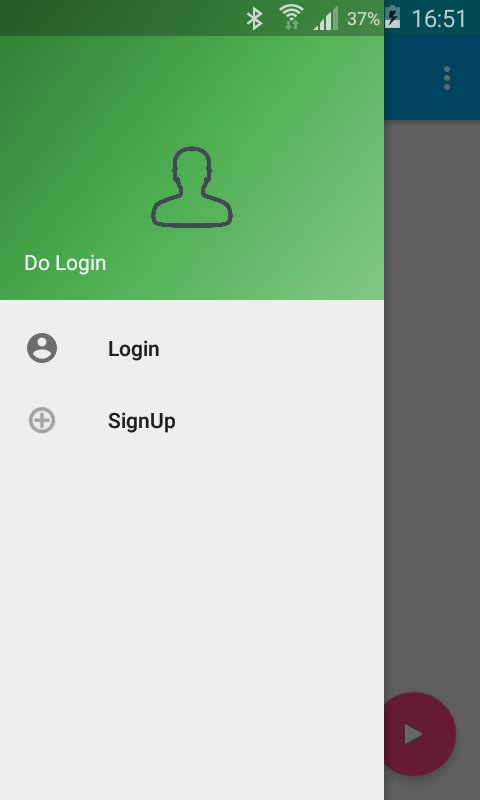
\includegraphics[height=0.3\textwidth]{imgs/left.png}
\caption[Menu lateral de Navegação]{Menu lateral de Navegação}
\label{f:leftpannel}
\end{figure}

\subsubsection{Atividade Principal}
O participante antes de efetuar Login tem a atividade Principal praticamente vazia. Pode aceder ao menu lateral (Figura \ref{f:leftpannel}), ou às configurações (Figura \ref{f:seesettings}).
\begin{figure}[H]
\centering
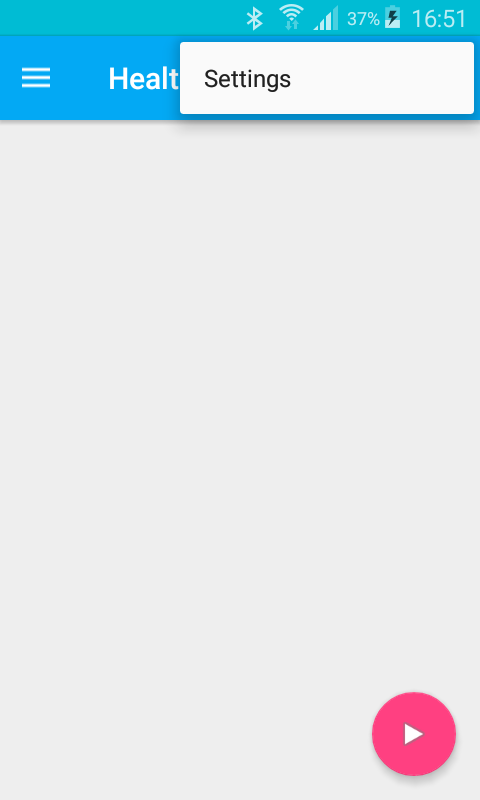
\includegraphics[height=0.3\textwidth]{imgs/seesettings.png}
\caption[Opção na atividade principal para abrir as configurações]{Opção na atividade principal para abrir as configurações}
\label{f:seesettings}
\end{figure}
Quando o participante efetua o Login na aplicação as suas sessões são carregadas e são listadas para que se possa verificar as medições efetuadas correspondentemente a cada uma. Na Figura \ref{f:afterlogin} podemos ver do lado esquerdo a situação em que o participante ainda não tem sessões de medições efetuadas e do lado direito quando já efetuou duas sessões de medições.

\begin{figure}[H]
\centering
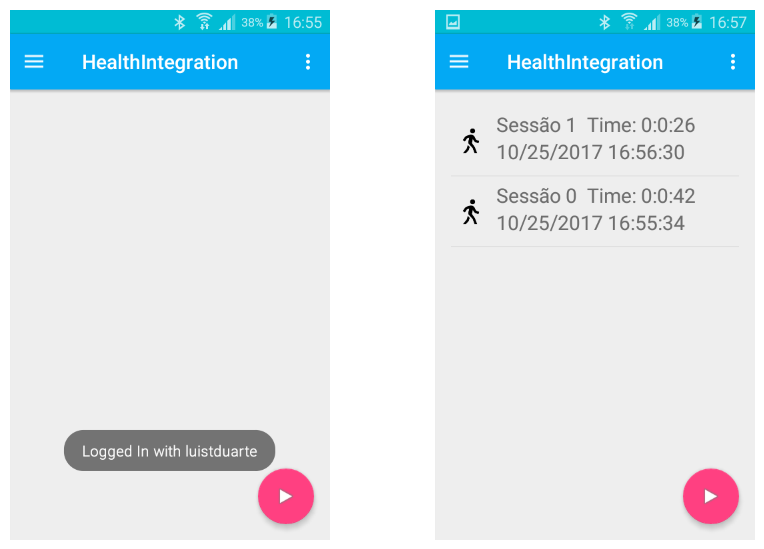
\includegraphics[height=0.4\textwidth]{imgs/afterlogin.png}
\caption[Atividade Principal depois do Login Efetuado]{Atividade Principal depois do Login Efetuado}
\label{f:afterlogin}
\end{figure}

\subsubsection{Atividade de Configurações}
Na atividade de configurações (Figura \ref{f:settings}) temos a possibilidade de: escolher o dispositivo que vai ser utilizado e ao qual se irá conectar; escolher tanto os tipos de dados que são para recolher como a sua relação temporal em relação à atividade física na altura que a medição está a ser efetuada.
\begin{figure}[H]
\centering
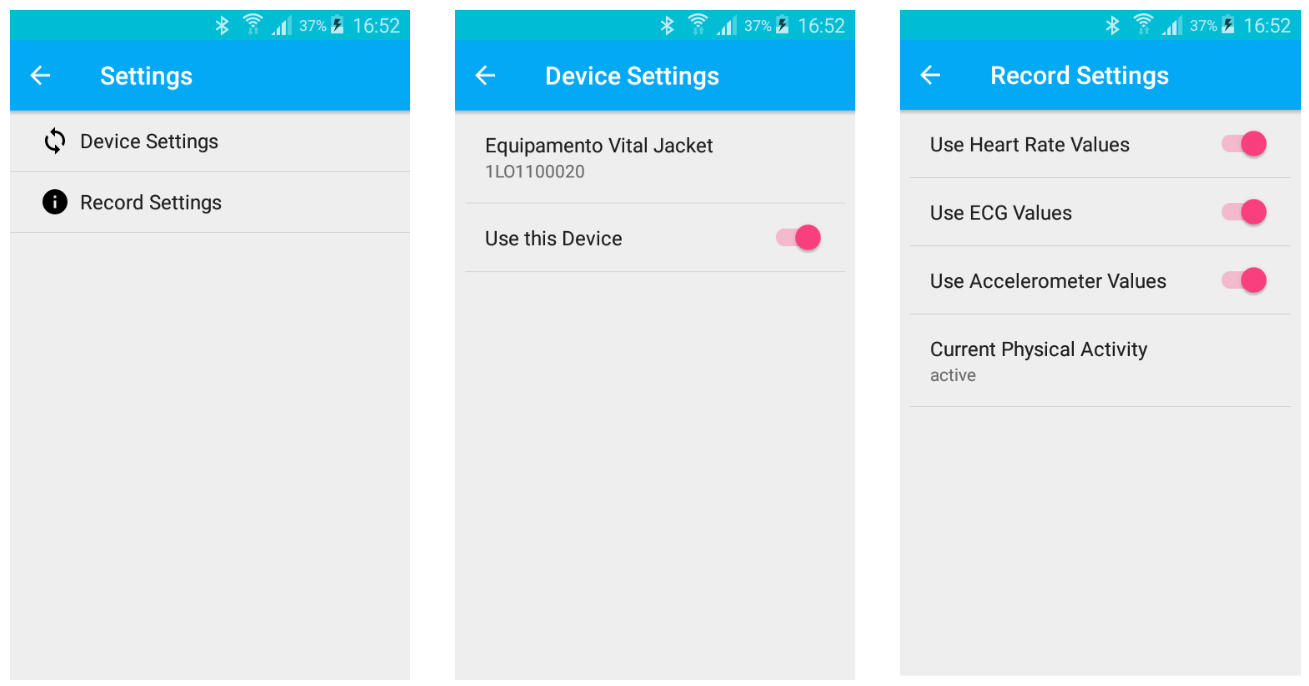
\includegraphics[height=0.6\textwidth]{imgs/settings.png}
\caption[Menu de Configurações e as respetivas opções de configuração]{Menu de Configurações e as respetivas opções de configuração}
\label{f:settings}
\end{figure}

\subsubsection{Atividade de Registo}
O participante pode ainda não ter uma conta criada, mas a possibilidade de criar uma conta existe na aplicação e está disponível através do menu lateral. No processo de criação de uma nova conta o participante tem que escolher um utilizador que ainda não tenha sido utilizado e escolher uma password para essa conta de utilizador(Figura \ref{f:createaccount}).
\begin{figure}[H]
\centering
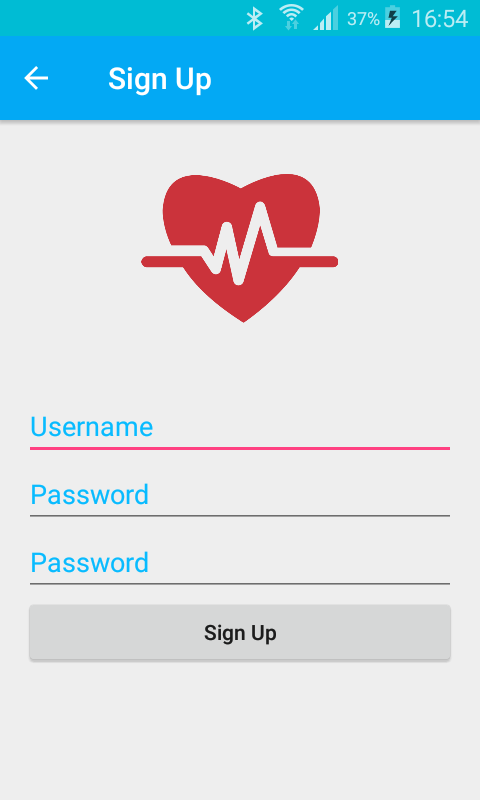
\includegraphics[height=0.3\textwidth]{imgs/signup_app.png}
\caption[Atividade para registo de um novo participante]{Atividade para registo de um novo participante}
\label{f:createaccount}
\end{figure}

\subsubsection{Atividade para efetuar o Login}
Esta atividade (Figura \ref{f:loginaccount}) pode ser chamada de duas duas maneiras diferentes: ao iniciar uma nova sessão de medições(é verificado que não tem login efetuado); escolhendo a opção para efetuar Login no menu lateral. É neste momento que o servidor de autorização e autenticação devolve um token de acesso.
\begin{figure}[H]
\centering
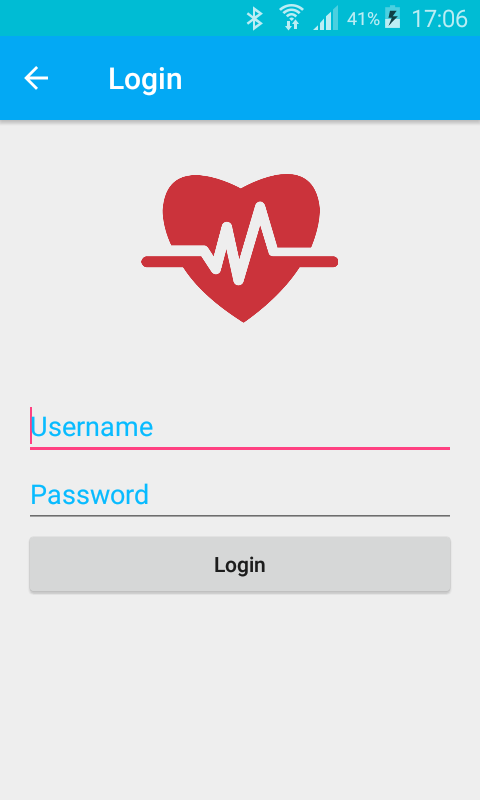
\includegraphics[height=0.3\textwidth]{imgs/before_login.png}
\caption[Atividade para efetuar o Login]{Atividade para efetuar o Login}
\label{f:loginaccount}
\end{figure}

\subsubsection{Atividade associada a uma nova sessão de leitura}
Depois de efetuar o login o participante pode então criar novas sessões de medições (Figura \ref{f:onNewSession}), pode parar quando quiser e irá voltar a visualizar a sua lista de medições com o acréscimo da última sessão efetuada. 
\begin{figure}[H]
\centering
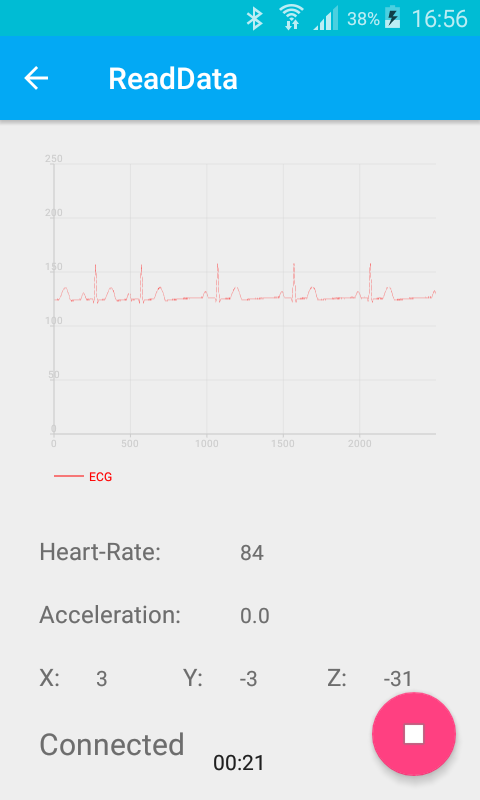
\includegraphics[height=0.3\textwidth]{imgs/reading.png}
\caption[Atividade relativa a uma nova sessão de medições]{Atividade relativa a uma nova sessão de medições}
\label{f:onNewSession}
\end{figure}

\subsubsection{Atividade Relativa a uma sessão}
Depois do participante ter entrado na aplicação com a sua conta pode visualizar as medições relativas a uma sessão, para isso basta clicar numa das sessões que compõem a lista. Nesta atividade (Figura \ref{f:read_data}) pode visualizar os dados relativos a cada tipo de medição, entre eles a frequência cardíaca, \gls{ECG} e acelerómetro, para isso tem disponível três diferentes separadores para mudar de tipo de medição. 
\begin{figure}[H]
\centering
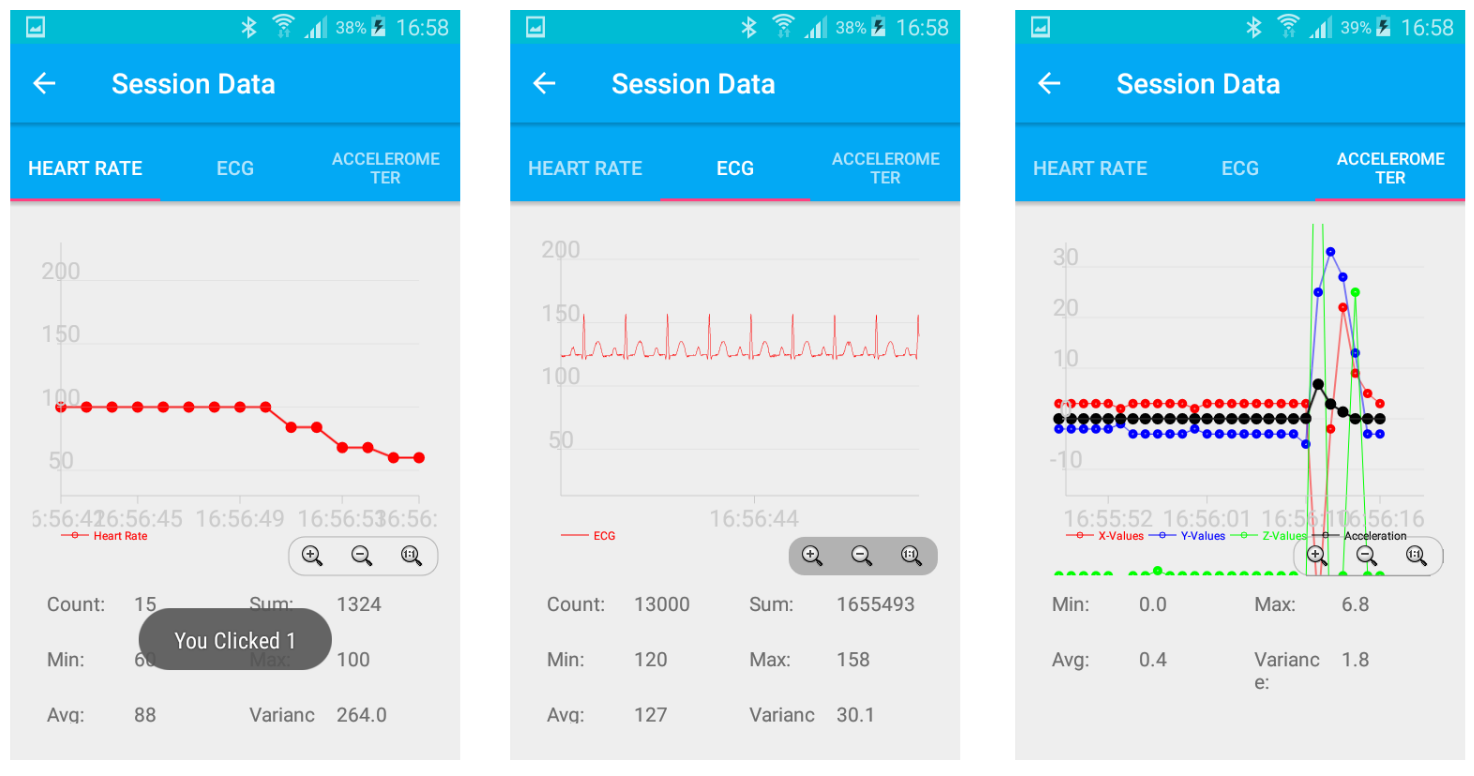
\includegraphics[height=0.4\textwidth]{imgs/read_data.png}
\caption[Atividade para visualizar os dados relacionados a uma determinada sessão]{Atividade para visualizar os dados relacionados a uma determinada sessão}
\label{f:read_data}
\end{figure}

\section{Implementação da aplicação de revisão}
\subsection{Tecnologias integradas e fontes de dados}

A aplicação web de revisão está a utilizar as \gls{API}s \gls{REST} definidas anteriormente em \ref{l:restapiAUTH} e em \ref{l:restapiRESOURCES}. Utiliza o serviço de autenticação e autorização para todas as interações envolvidas com registo, login e acesso aos dados. O serviço de recursos é utilizado para consultar todas as medições efetuadas pelos participantes em estudo e para guardar os dados demográficos de cada participante adicionado ao seu estudo.\par

\subsection{Componentes da aplicação}
Esta aplicação foi desenvolvida como aplicação web com recurso a \gls{HTML} Java Script e \gls{CSS}. \par 
Foi utilizada a framework Bootstrap \cite{bootstrap} da versão 3.3.7 que fornece uma base em \gls{HTML} e \gls{CSS} muito popular no mundo das aplicações web para desenvolvimento responsivo adaptável a plataformas móveis. \par
Para a comunicação com a \gls{API} \gls{REST} foi utilizado o jQuery \cite{jquery}.
Relativamente à visualização dos dados para cada sessão foi utilizado a bilbioteca HighCharts \cite{highcharts} para a visualização dos dados relacionados com o acelerómetro e \gls{ECG}. Para a frequência cardíaca decidimos utilizar um visualizador padrão desenvolvido pela \gls{OMH} denominado de Open mHealth Web Visualizations \cite{omhwebvisualizations}.

\subsection{Interações suportadas }


Esta aplicação móvel foi desenvolvida com o objetivo principal de efetuar a revisão dos dados inseridos pelos participantes. É então possível adicionar vários participantes e verificar as várias sessões de medições de dados.
\subsubsection{Página Principal}
A página principal tem uma secção de boas vindas e ainda permite a criação e a entrada na aplicação (Figura \ref{f:web-home}).

\begin{figure}[H]
\centering
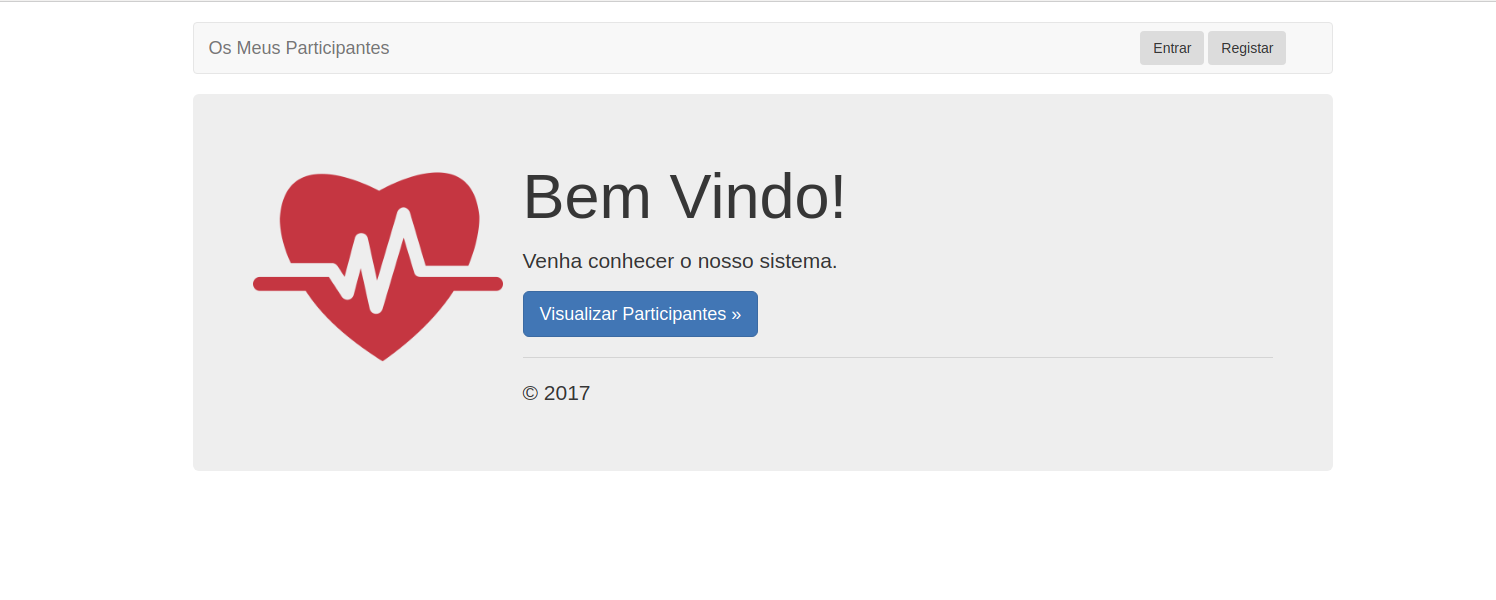
\includegraphics[width=1\textwidth]{imgs/home.png}
\caption[Página principal da aplicação de revisão]{Página principal da aplicação de revisão}
\label{f:web-home}
\end{figure}

\subsubsection{Página de Registo}
O revisor pode ainda não ter uma conta criada, por isso antes de entrar na aplicação terá que efetuar o registo de uma nova conta. Na criação é necessário escolher uma nova conta que ainda não tenha sido utilizada acompanhada de uma password (Figura \ref{f:web-registo}).

\begin{figure}[H]
\centering
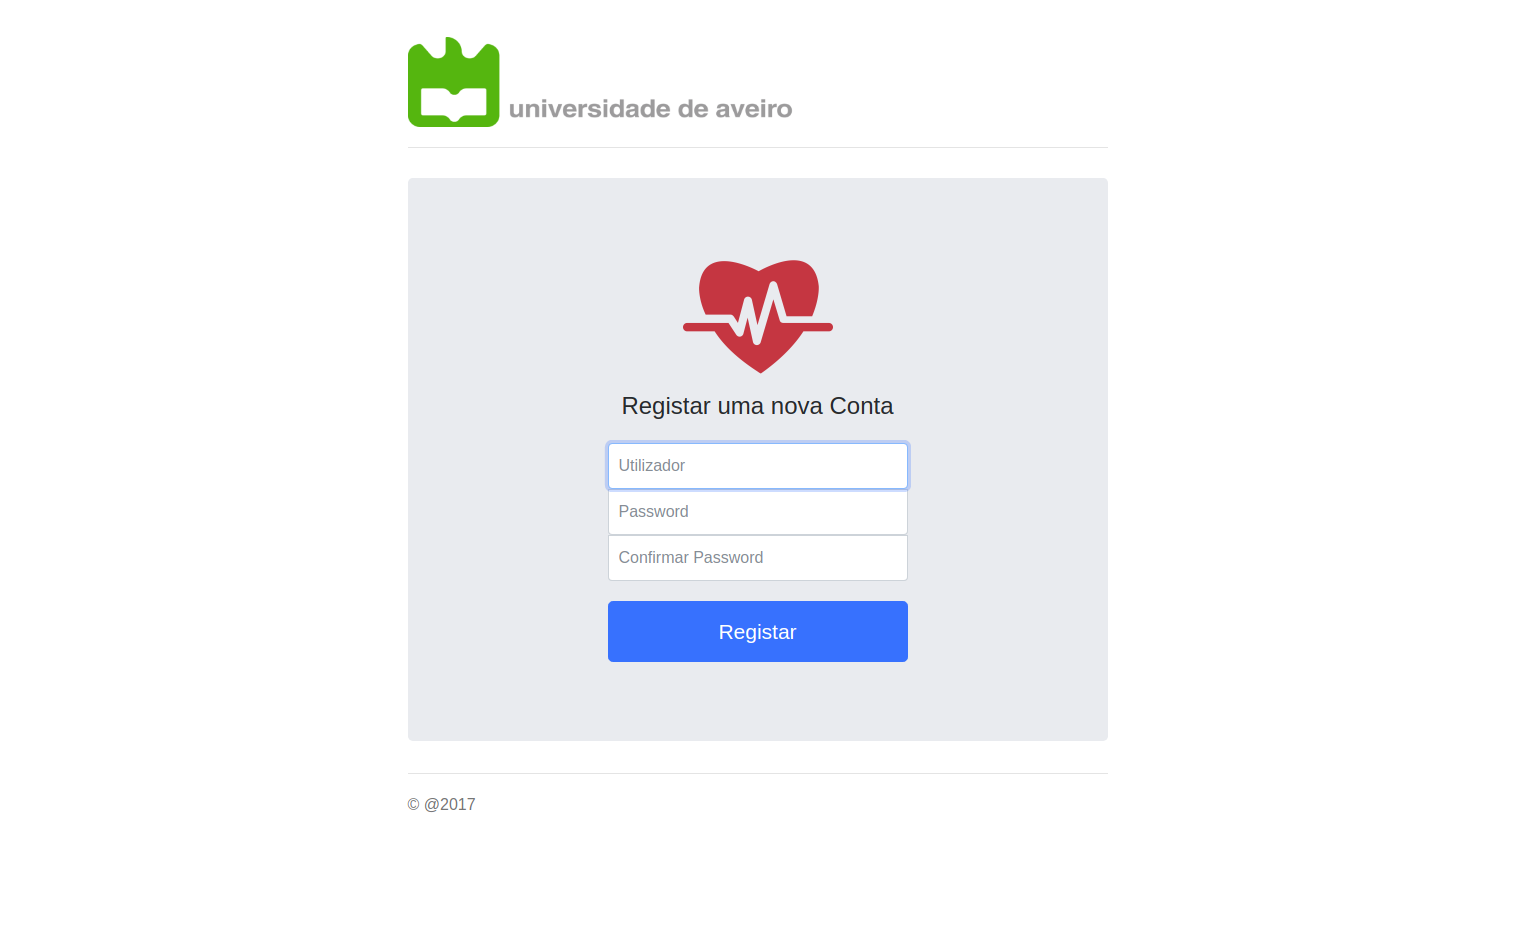
\includegraphics[width=1\textwidth]{imgs/signup_web.png}
\caption[Página de registo na aplicação de revisão]{Página de registo na aplicação de revisão}
\label{f:web-registo}
\end{figure}

\subsubsection{Página para efetuar o Login}
Esta página permite (Figura \ref{f:web-login}) pode ser chamada de duas maneiras diferentes. Ao clicar nos participantes da secção de boas vindas é detetado que o login ainda não foi efetuado e é feito o redirecionamento para esta página, ou então ao clicar no botão Entrar na página principal. Depois de efetuar o login pode visualizar os seus participantes.

\begin{figure}[H]
\centering
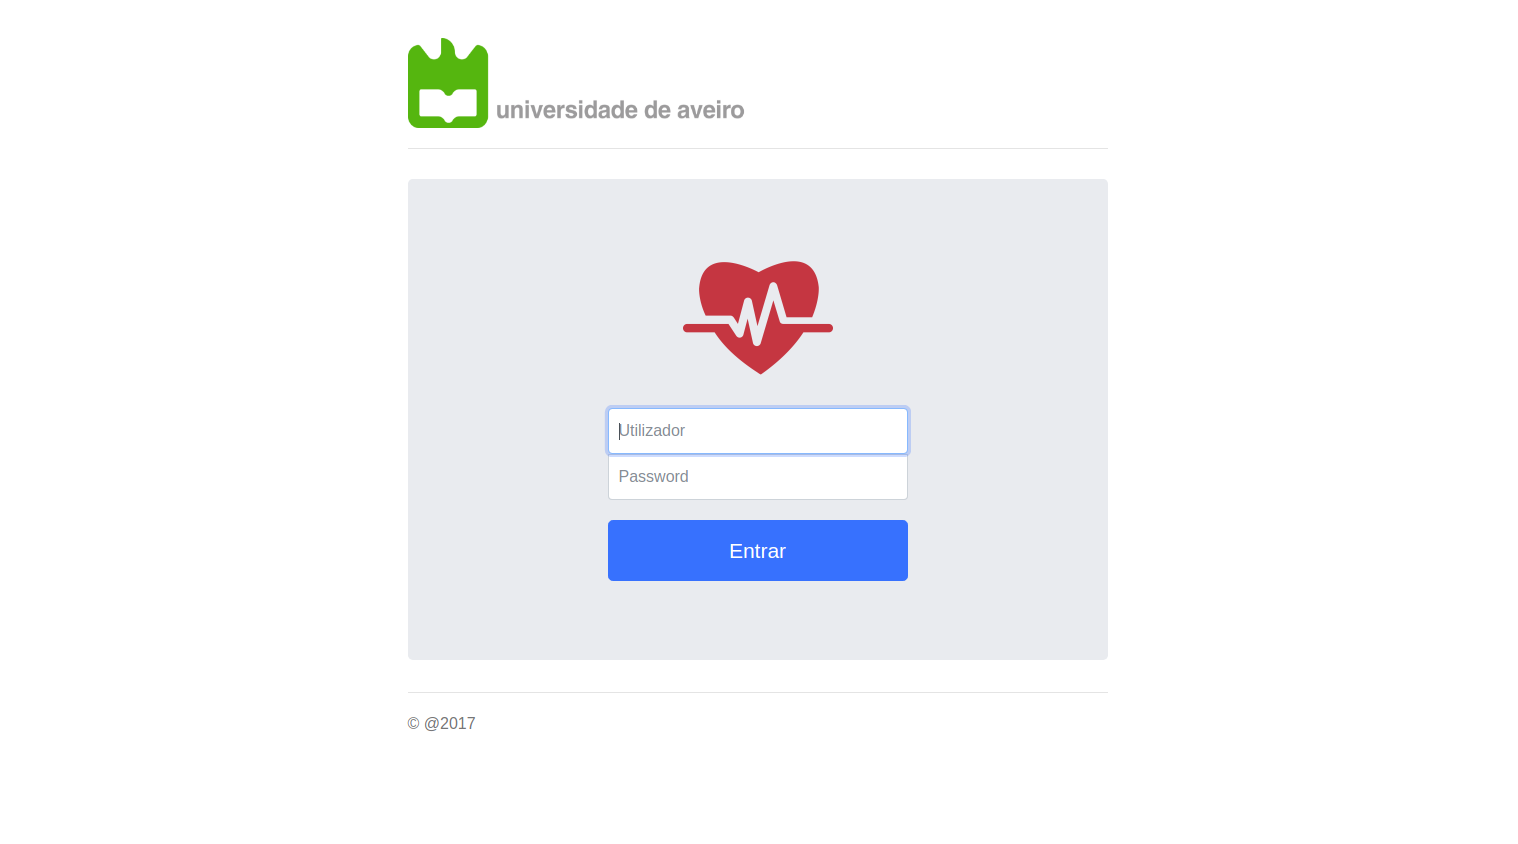
\includegraphics[width=1\textwidth]{imgs/login_web.png}
\caption[Página de login na aplicação de revisão]{Página de login na aplicação de revisão}
\label{f:web-login}
\end{figure}

\subsubsection{Página com todos os participantes}
Esta página é composta por uma grelha onde pode visualizar todos os seus participantes e também adicionar novos participantes. Assim que são adicionados novos participantes a grelha vai ficando mais composta, como na Figura \ref{f:gridParticipante}

\begin{figure}[H]
\centering
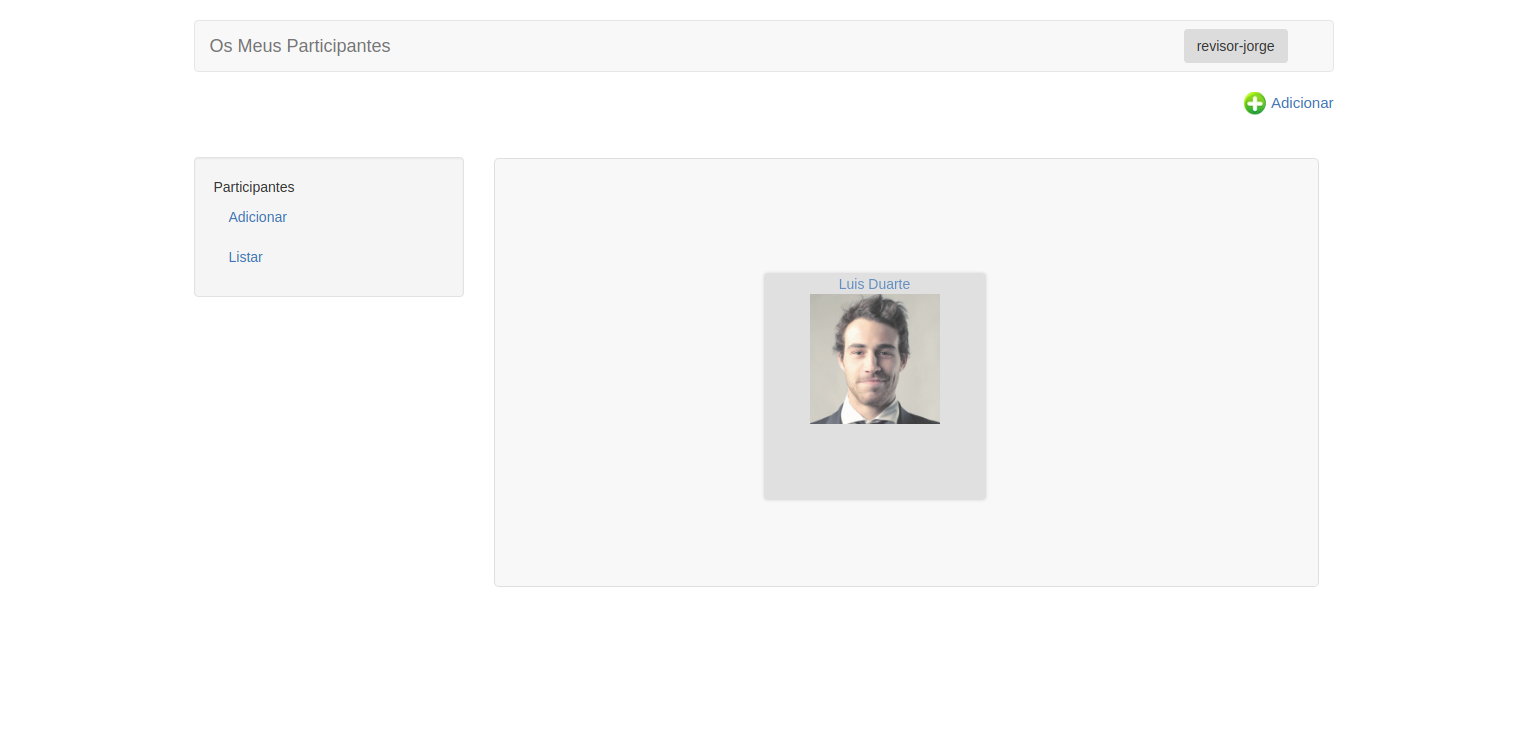
\includegraphics[width=0.9\textwidth]{imgs/list_after_add_web.png}
\caption[Página com grelha de participantes]{Página com grelha de participantes}
\label{f:gridParticipante}
\end{figure}


\subsubsection{Página para adicionar novo participante}
Nesta página (Figura \ref{f:web-newparticipante}) pode adicionar um novo participante, para isso tem que identificar o username do participante e todos os dados demográficos disponíveis deste participante. Depois de adicionar vai ser redirecionado para a página relativa a todos os participantes. 

\begin{figure}[H]
\centering
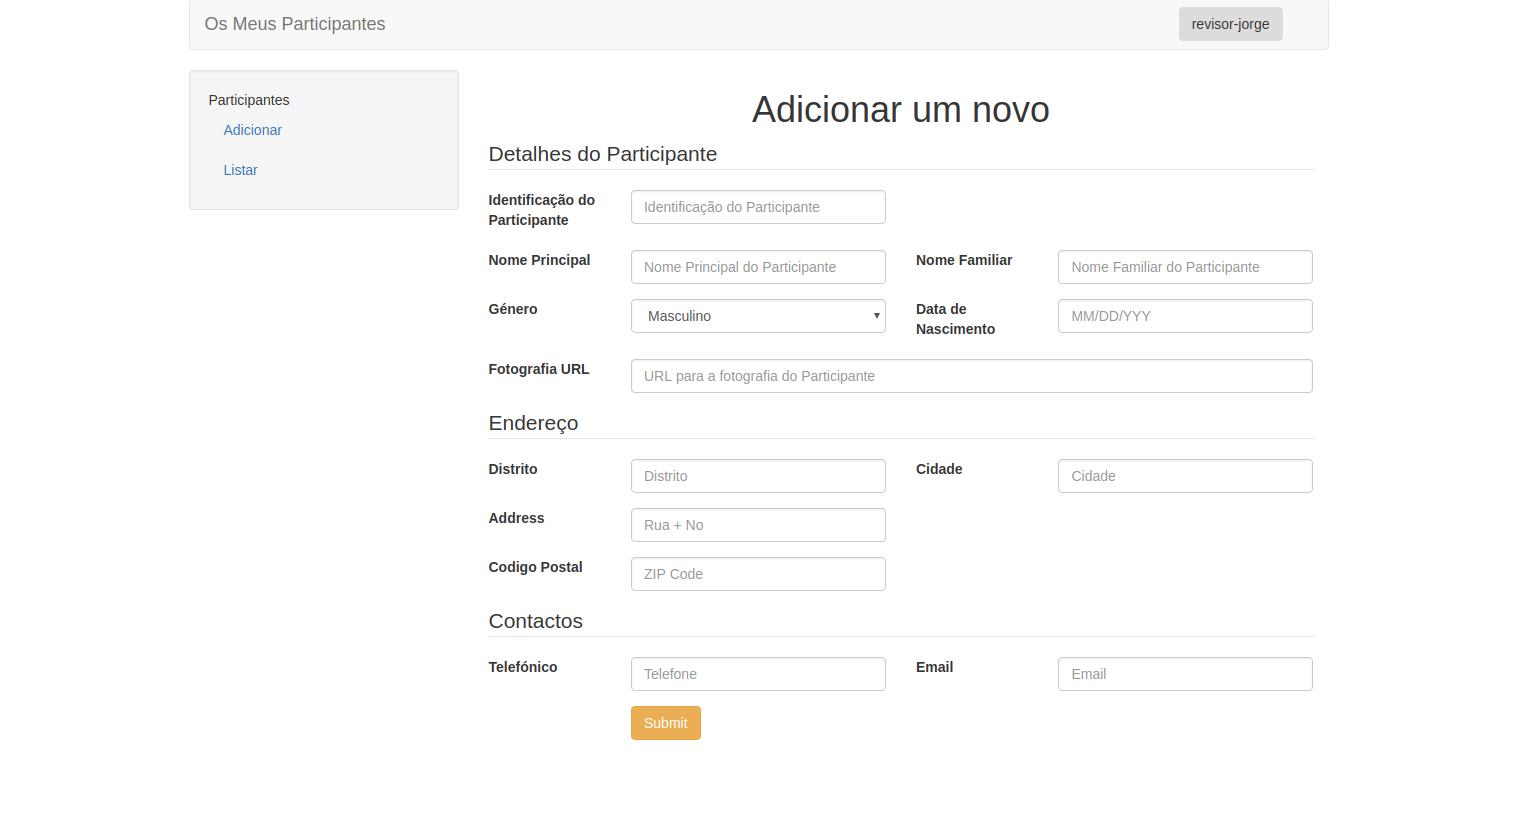
\includegraphics[width=1\textwidth]{imgs/add_participant_web.png}
\caption[Página para adicionar novo participante ao estudo]{Página para adicionar novo participante ao estudo}
\label{f:web-newparticipante}
\end{figure}
\newpage
\subsubsection{Página com leituras do participante}
Nesta página pode visualizar todos os dados demográficos e fisiológicos do participante. Os dados demográficos podem ser atualizados e os dados fisiológicos que podem ser consultados são todos aqueles inseridos pelo participante. Para isso terá que escolher um intervalo de datas para procurar por sessões de leitura nesse intervalo, depois disso as várias sessões compõem um dropdow menu (Figura \ref{f:webleiturassessoes}) onde pode escolher a sessão que pretende rever. 

\begin{figure}[H]
\centering
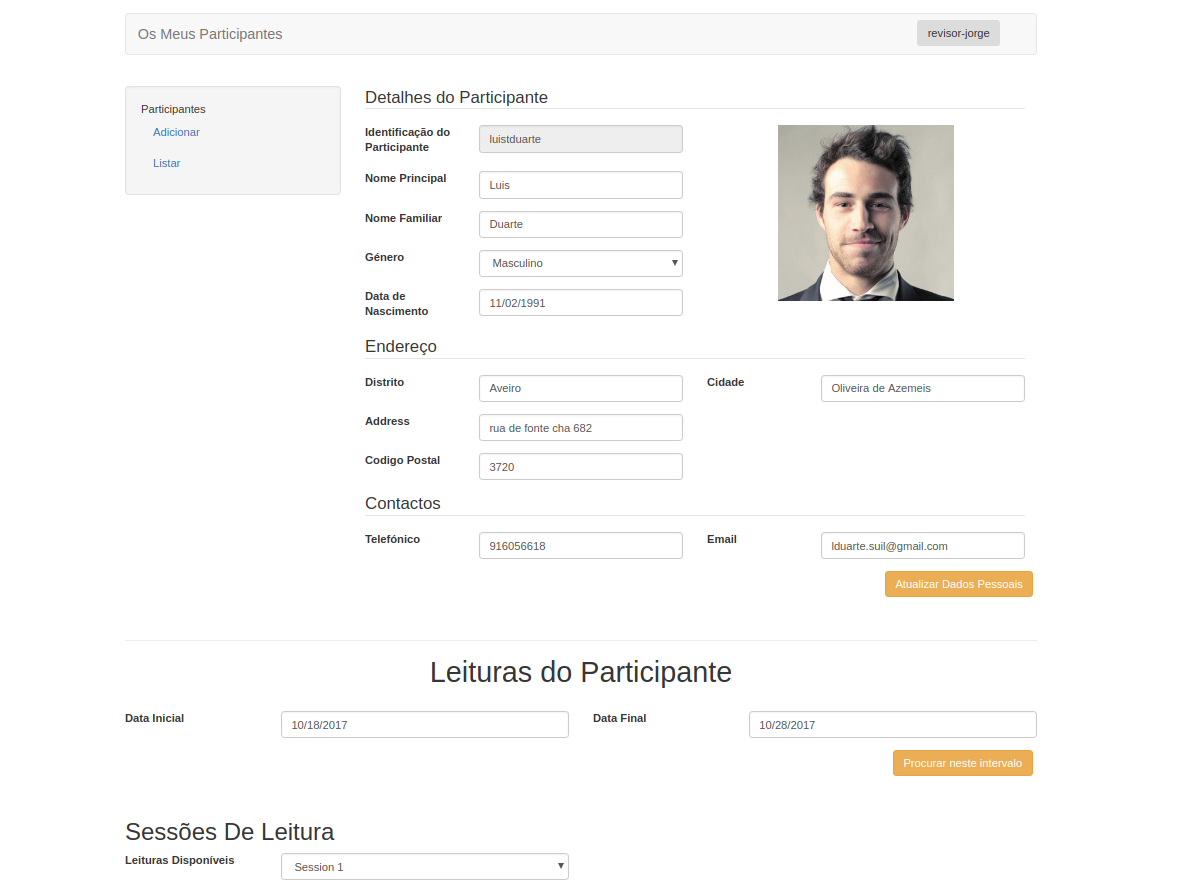
\includegraphics[width=1\textwidth]{imgs/user-info-web.png}
\caption[Página com dados demográficos e fisiológicos do participante]{Página com dados demográficos e fisiológicos do participante}
\label{f:webleiturassessoes}
\end{figure}

Podemos então visualizar os dados em gráficos relativos a cada tipo de dados recolhido (Figura \ref{f:leiturasdados}). 

\begin{figure}[H]
\centering
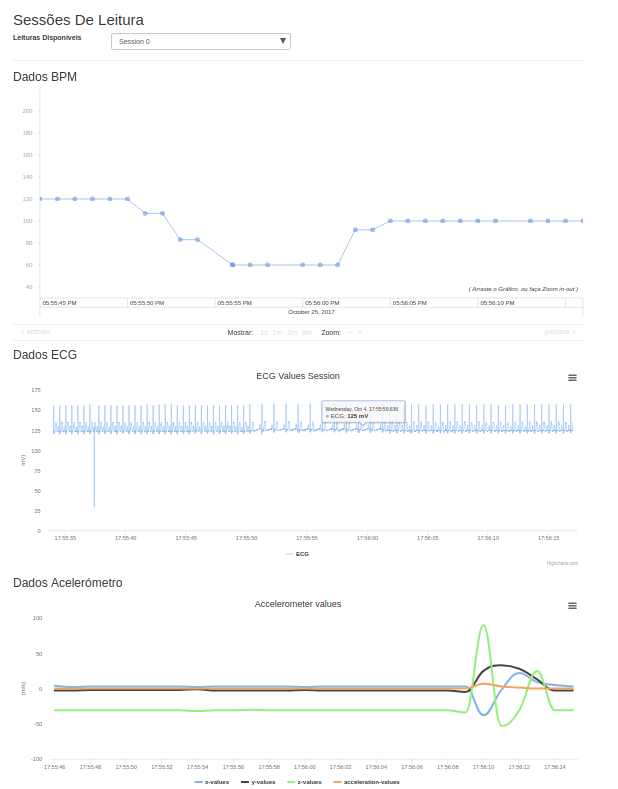
\includegraphics[width=1\textwidth]{imgs/dadosfisiologicos-web.png}
\caption[Dados fisiológicos do participante numa determinada sessão]{Dados fisiológicos do participante numa determinada sessão}
\label{f:leiturasdados}
\end{figure}
 Relativamente a cada tipo de dados pode ser efetuado o zoom para em cada um dos gráficos, e ainda no caso do acelerómetro escolher os dados a apresentar, neste caso escolhi apenas a aceleração (Figura \ref{f:withzoom}).
 
 \begin{figure}[H]
\centering
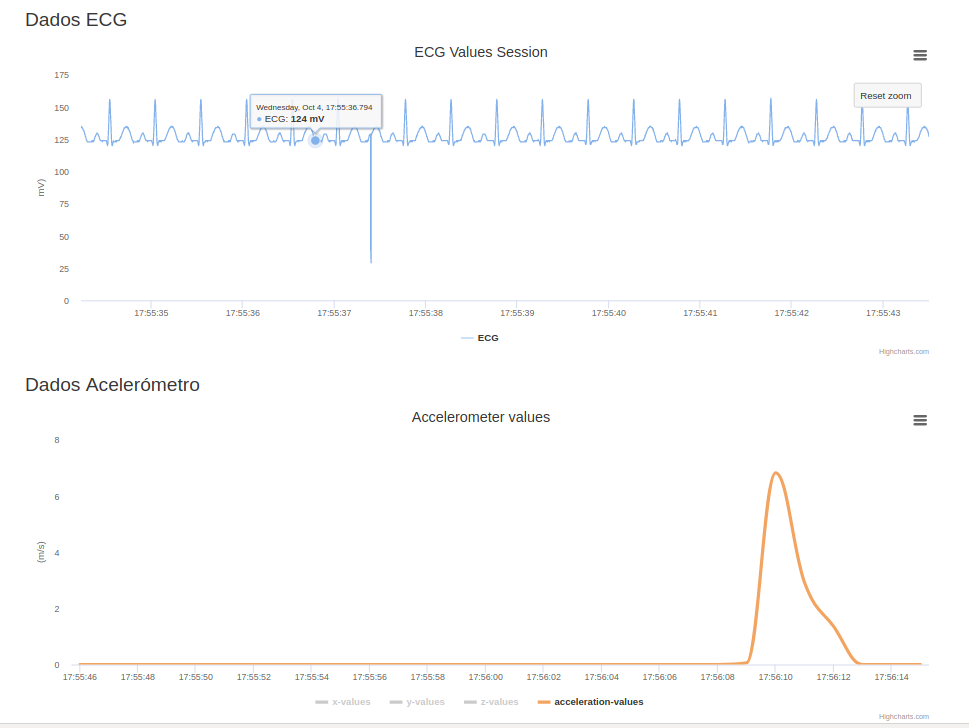
\includegraphics[width=1\textwidth]{imgs/withzoom-choosen-web.png}
\caption[Dados fisiológicos do participante mais detalhados]{Dados fisiológicos do participante mais detalhados}
\label{f:withzoom}
 \end{figure}
\section{Como aplicar e estender a plataforma em novos contextos}

% explicar como se pega no que ficou feito para usar num novo projeto e como se pode estender (e.g: para novos tipos de dados)

\subsection{Criar um novo tipo de dados}

A criação de um novo tipo de dados pode ser feita com a ajuda do repositório ''schemas'' \cite{schemas-rep} que foi criado pela organização da \gls{OMH}. Para isto vai necessitar de algumas ferramentas entre elas: o git \cite{git-install} para puxar o repositório; o Java 8 \cite{java-overview} para executar o validador; um editor de texto como por exemplo o atom \cite{atom-install}. Vou descrever agora a lista de tarefas para conseguir efetuar a criação de um novo tipo de dados. Para este tutorial vou criar o tipo de dados acelerómetro. É um dos tipos de dados que são obtidos através do VitalJacket.

\begin{enumerate}
  \item Clonar o repositório correspondente para um diretório à sua escolha com o comando \par
  ''git clone https://github.com/openmhealth/schemas'' 
  De seguida vamos fazer duas coisas principais: uma delas é criar o ficheiro que define o novo tipo de dados; a outra é criar um ficheiro com uma amostra do novo tipo de dados.
  \item Criar um ficheiro que define o tipo de dados em \gls{JSON} schema, para isso, adicione um novo ficheiro no diretório schema/omh. O nome deste ficheiro tem que ser composto pelo nome que quer dar ao tipo de dados e a versão correspondente, tem que terminar com a extensão .json. No meu caso criei com o nome accelerometer-1.0.json  \par A versão escolhida aqui é a 1.0 mas podia ser qualquer outra. Pode reparar que no diretório schema/omh tem acesso a todos os ficheiros que definem todos os tipos de dados.
  \item Adicionar uma nova pasta ao diretório testdata/omh como o nome respetivo ao ficheiro criado anteriormente. Neste caso criar uma pasta com o nome accelerometer.
  \item Vai agora criar uma pasta correspondente à versão introduzida no ponto 2. Neste caso é 1.0 e uma outra pasta dentro da criada anteriormente com o nome shouldPass.
  \item Dentro do diretório shouldPass vai ter que criar um ou vários ficheiros para ser utilizados como amostras do tipo de dados. O objetivo deste diretório é ter várias amostras válidas testando-as com o tipo de dados criado no ponto 2. Para este tutorial criei o ficheiro example.json. \par Neste ponto o nome do ficheiro é opcional só tem que acabar com a extensão .json
  Como criou o diretório shouldPass, pode também criar o diretório shouldFail criando também vários ficheiros para testar o tipo de dados criado. \par 
  Neste ponto tem tudo preparado para começar a criar o novo tipo de dados e validar a amostra com a nova definição do novo tipo de dados criados.
  
  \begin{figure}[!ht]
  \centering
  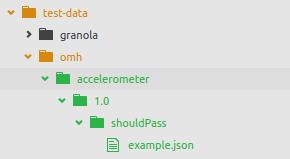
\includegraphics[width=0.5\textwidth]{imgs/newsampledata.png}
  \caption[Esquema de diretório para o novo sample]{Esquema de diretório para o exemplo do novo tipo de dados}
  
  \label{f:directorynewsample}
\end{figure}
  
\item Vamos agora preencher o ficheiro com a definição do novo tipo de dados, aquele que criou no ponto 2. O ficheiro vai ser criado no formato de \gls{JSON} schema. Para suportar a criação deste ficheiro pode reutilizar schemas existentes \cite{schema-library} e referênciá-los, deste modo estará a criar um modelo com tipos de dados normalizados. No meu caso vou reutilizar um schema para definir a data/hora e um outro para definir o tipo de atividade que está a efetuar no momento da leitura. Os restantes dados estão relacionados com o acelerómetro em si, a sessão e a leitura respetiva.
O ficheiro fica do seguinte modo: 

\begin{figure}[H]
\inputminted[fontsize=\scriptsize]{json}{code/accelerometer-1.0.json}
\caption[\gls{JSON} schema para o novo tipo de dados de acelerómetro]{\gls{JSON} schema para o novo tipo de dados de acelerómetro}
\label{f:accelerometer-json-schema}
\end{figure}

\item Preencha o ficheiro com uma amostra do novo tipo de dados, para isso tem que ter em conta a definição utilizada, pois porque se esta amostra não for compatível não vai passar no validador.

\begin{figure}[H]
\inputminted[fontsize=\scriptsize]{json}{code/example.json}
\caption[Exemplo do tipo de dados de acelerómetro]{Exemplo do tipo de dados de acelerómetro}
\label{f:accelerometer-json-data}
\end{figure}

\item Para compilar e executar o validador tem que executar o comando ''./gradlew test-data-validator:bootRun'' no diretório principal ''schemas'' ou então execute o comando ''./gradlew bootRun'' no diretório ''schemas/test-data-validator''. 

\subsection{Como utilizar o novo tipo de dados criado}

Para adicionar o novo tipo de dados criado, tem que o integrar com os restantes tipos de dados existentes. \par Tendo em conta que já tem o repositório omh-dsu-ri clonado através do comando ''git clone https://github.com/luistduarte/omh-dsu-ri', terá que copiar o seu novo tipo de dados para o diretório ''omh-dsu-ri/resource-server/src/main/resources/schema/omh'' que é onde se encontram os restantes tipos de dados válidos.

\end{enumerate}

\cleardoublepage
